%%% LaTeX Template: Two column article
%%%
%%% Source: http://www.howtotex.com/
%%% Feel free to distribute this template, but please keep to referal to http://www.howtotex.com/ here.
%%% Date: February 2011

%%% Preamble
\documentclass[	DIV=calc,%
							paper=a4,%
							fontsize=12pt,%
							onecolumn]{scrartcl}% KOMA-article class
\usepackage{placeins}
\usepackage{longtable}
\usepackage{multirow}
\usepackage{lipsum}	% Package to create dummy text
\usepackage[brazil]{babel}										% English language/hyphenation
\usepackage[protrusion=true,expansion=true]{microtype}				% Better typography
\usepackage{amsmath,amsfonts,amsthm}					% Math packages
\usepackage[pdftex]{graphicx}									% Enable pdflatex
\usepackage[svgnames]{xcolor}									% Enabling colors by their 'svgnames'
\usepackage[hang, small,labelfont=bf,up,textfont=it,up]{caption}	% Custom captions under/above floats
\usepackage{epstopdf}												% Converts .eps to .pdf
\usepackage{subfig}													% Subfigures
\usepackage{booktabs}												% Nicer tables
\usepackage{fix-cm}													% Custom fontsizes
\usepackage[utf8]{inputenc}
\usepackage[top=2.5cm, bottom=2.5cm, left=2.5cm, right=2.5cm]{geometry}
\usepackage[ddmmyyyy]{datetime}
\addto\captionsenglish{%
	\renewcommand\tablename{Tabela}
	\renewcommand\figurename{Figura}
} 

%%% Custom sectioning (sectsty package)
\usepackage{sectsty}													% Custom sectioning (see below)
\allsectionsfont{%															% Change font of al section commands
	\usefont{OT1}{phv}{b}{n}%										% bch-b-n: CharterBT-Bold font
	}

\sectionfont{%																% Change font of \section command
	\usefont{OT1}{phv}{b}{n}%										% bch-b-n: CharterBT-Bold font
	}



%%% Headers and footers
\usepackage{fancyhdr}												% Needed to define custom headers/footers
	\pagestyle{fancy}														% Enabling the custom headers/footers
\usepackage{lastpage}	

% Header (empty)
\lhead{}
\chead{}
\rhead{}
% Footer (you may change this to your own needs)

%% ====================================
%% ====================================
%% mude o rodape  do projeto
%% ====================================
%% ====================================

\lfoot{\footnotesize \texttt{Template para entrega de texto} \textbullet ~Modelo de projeto}


\cfoot{}
\rfoot{\footnotesize página \thepage\ de \pageref{LastPage}}	% "Page 1 of 2"
\renewcommand{\headrulewidth}{0.0pt}
\renewcommand{\footrulewidth}{0.4pt}



%%% Creating an initial of the very first character of the content
\usepackage{lettrine}
\newcommand{\initial}[1]{%
     \lettrine[lines=3,lhang=0.3,nindent=0em]{
     				\color{DarkGoldenrod}
     				{\textsf{#1}}}{}}
%%% Title, author and date metadata
\usepackage{titling}															% For custom titles

\newcommand{\HorRule}{\color{DarkGoldenrod}%			% Creating a horizontal rule
									  	\rule{\linewidth}{1pt}%
										}

\pretitle{\vspace{-30pt} \begin{flushleft} \HorRule 
				\fontsize{50}{50} \usefont{OT1}{phv}{b}{n} \color{DarkRed} \selectfont 
				}

%% ====================================
%% ====================================
%% mude o titulo  do projeto
%% ====================================
%% ====================================

\title{Modelo de Processo S.C.U. }					% Title of your article goes here

%% ====================================



\posttitle{\par\end{flushleft}\vskip 0.5em}

\preauthor{\begin{flushleft}
					\large \lineskip 0.5em \usefont{OT1}{phv}{b}{sl} \color{DarkRed}}
\author{Felipe Issamu de Melo Kamimura, Isabelle Ichikawa Yagi, Lucas Freitas Costa, Lucas Tarumoto, Nathiely Moraes Macedo, Raniel Carlos Bispo dos Santos }  	% Author name goes here


\postauthor{\footnotesize \usefont{OT1}{phv}{m}{sl} \color{Black} 
					\\Universidade Tecnológica Federal do Paraná - Campus Cornélio Procópio 								% Institution of author
					\par\end{flushleft}\HorRule}

\date{}																				% No date




%%% Begin document
\begin{document}
\maketitle
\thispagestyle{fancy} 	
\thispagestyle{empty}		% Enabling the custom headers/footers for the first page 
% The first character should be within \initial{}




%% ====================================
%% ====================================
%% mude o resumo  do projeto
%% ====================================
%% ====================================
\initial{E}\textbf{ste documento descreve um modelo de processo de desenvolvimento de Software S.C.U.}

%% ====================================
\begin{figure}
	\centering
	
\includegraphics{utfpr}
\end{figure}

\vspace{3cm}
\centerline{\textit{\textbf{\today}}}

\clearpage
    \renewcommand*\listfigurename{Lista de figuras}
\listoffigures

\renewcommand*\listtablename{Lista de tabelas}
\listoftables




\clearpage
\renewcommand{\contentsname}{Sumário}
\tableofcontents
\clearpage

%% ====================================
%% ====================================
%% Inicio do texto
%% ====================================
%% ====================================
\section{Introdução}
O presente documento descreve um processo de produção de software construído com base no Scrum \cite{sutherland2014scrum}, no Cascata \cite{sommervilleengenharia} e no Processo Unificado \cite{scott2003processo}, o SCU, que busca unir conceitos de metodologia ágil com metodologia clássica, o objetivo é um processo simples de coordenar e bastante interativo, onde a comunicação entre os envolvidos e o comprometimento com cada fase do processo são evidenciados ao longo do desenvolvimento.	

Assim os integrantes que realizarão o projeto serão estes apresentados a seguir, cada um com seu respectivo papel:


\begin{itemize}
	\item Felipe Kamimura - Integrante do Scrum Team
	\item Isabelle Ichikawa - Scrum Master
	\item Lucas Freitas - Integrante do Scrum Team
	\item Lucas Tarumoto - Integrante do Scrum Team
	\item Nathiely Moraes - Integrante do Scrum Team
    \item Raniel Santos - Integrante do Scrum Team
\end{itemize}

O Product Owner deve ser o cliente do projeto que será desenvolvido utilizando o processo SCU. Oendereço do repositório do projeto é: \\
https://github.com/FelipeKamimura/GerenciaDeConfig-SCU.


\section{Processo}

O processo foi implementado com elementos do Scrum \cite{sutherland2014scrum}, do Processo Unificado \cite{scott2003processo} e do modelo Cascata \cite{sommervilleengenharia}. As fases constantes no cascata \cite{sommervilleengenharia} foram mantidas no SCU, sendo consideradas sprints, que possuem reuniões no início de cada fase, onde são discutidos os objetivos da sprint, as dificuldades encontradas no desenvolvimento da sprint anterior e os avanços alcançados (conforme templates de reuniões).

Para garantir que o processo tenha qualidade, assim como o scrum, o processo proposto segue as diretrizes do modelo de qualidade CMMI, pois se trata de uma metodologia ágil. Este modelo requer padronização nos processos, sendo assim, todas as fases do SCU são definidas nesse documento, além dos relatórios e reuniões que possuem um padrão de documentação aqui disponibilizados. O planejamento dos prazos também são detalhados neste documento, a fim de tornar o processo gerenciado. O processo atende às requisições de definido, sendo descrito detalhadamente todos os seus procedimentos no presente documento.

Do processo unificado foram extraídos os artefatos e os papéis \cite{scott2003processo}, entretanto os papéis do scrum \cite{sutherland2014scrum}também fazem parte do processo, sendo eles o Scrum Master, Product Owner e Scrum Team \cite{sutherland2014scrum} (os papéis são detalhados no item 2.1 deste documento. Além das sprints tradicionais do Scrum \cite{sutherland2014scrum}, no SCU existem as subsprints, que são conjuntos de atividades, podendo ser feitas em paralelo ou não, com determinado prazo de entrega. A diferenciação em sprints e subsprints se deve às reuniões, pois as sprints dependem das reuniões realizadas antes de sua iniciação, já as subsprints não possuem reuniões formais. A retroatividade do modelo cascata também é mantida, dessa forma, caso haja mudanças nos requisitos, por exemplo, pode-se voltar pra primeira fase e realizar as alterações.

A primeira coisa a ser realizada no processo é a reunião de iniciação, o objetivo desta reunião é envolver todos os stakeholders no processo, é o momento em que o Scrum Master mostra o contexto do projeto para sua equipe e orienta os membros em relação às suas atividades, em seguidas as subsprints são definidas e o prazo de entrega estipulado.

Após realizar a reunião de iniciação, dá-se o início das Sprints, que são as fases do modelo cascata. A primeira fase se trata do Levantamento de Requisitos \cite{sommervilleengenharia}, que é formado por cinco subsprints com um total de duração de 6 semanas. O longo prazo dessa fase se deve a complexidade das subsprints, os requisitos são fundamentais para o sucesso do projeto, portanto o foco nessa parte do processo é muito importante. As subsprints e suas atividades podem ser visualizadas no item 3 deste documento, os artefatos gerados estão no item 3.2.

Ao final das 6 semanas, é realizada a reunião de iniciação sprint, a organização que adota o processo define como serão realizadas as reuniões, não existe nenhuma obrigatoriedade quanto à duração ou permanecer em pé como acontece no scrum, o único requisito é que seja documentada conforme o template disponibilizado.

Com a reunião concluída e documentada, é iniciada a segunda Sprint, que é a fase de Projeto e Implementação do cascata \cite{sommervilleengenharia}, é importante ressaltar que os integrantes da equipe (definido pelo Scrum Team) podem assumir diferentes funções ao longo do processo. Esta fase tem a duração de 7 semanas com 3 subsprints, sendo 4 semanas reservadas para a subsprint de implementação, que consiste na codificação e descrição do código do sistema. Ao final da sprint, novamente é realizada uma reunião de iniciação da sprint.

A terceira sprint do SCU é a fase de Verificação e Validação , com a duração de 2 semanas, essa fase é rápida, porém deve ser realizada com muita atenção, é nela que serão identificados os problemas decorrentes no sistema por meio de testes que devem ser executados com base num conjunto de casos de teste definidos pela organização/Scrum master juntamente com a equipe, que é o plano de teste. Esta fase pode identificar mudanças nos requisitos, por isso é importante realizar uma avaliação dos testes, que ajuda a decidir se essas mudanças são realmente plausíveis, pois nada impede que um teste seja conduzido incorretamente levando a resultados incoerentes com o objetivo da aplicação. Ao esgotar o prazo da sprint e concluir os testes, é o momento de realizar a reunião e dar início a quarta sprint.

A próxima sprint consiste na fase de Implantação do cascata \cite{sommervilleengenharia}, no SCU é estabelecida num período de 2 semanas, com 4 subsprints definidas. Nessa parte do processo o sistema é disponibilizado para os usuários, portanto deve ser entregue um manual e os treinamentos devem ser realizados para utilização do software, além disso, a instalação deve ser documentada conforme o relatório de instalação disponibilizado, isto é importante para controlar a distribuição do sistema. A utilização do sistema pelos usuários pode acarretar em novas mudanças ou aparecimento de bugs, essas informações devem constar no relatório de implantação ou ser discutidas e documentadas na reunião para iniciação da próxima Sprint.

A última sprint é a fase de Manutenção e Evolução do cascata \cite{sommervilleengenharia}, essa fase possui 5 subsprints, a subsprint chamada “gerência de alteração” tem a duração de 2 semanas, é nela que são corrigidos bugs percebidos durante a utilização do sistema e adotadas rotinas para manutenção e testes constantes do produto. Além disso, essa sprint controla as versões do sistema, as possíveis alterações e informações relacionadas ao progresso e resultados do software, as subsprints responsáveis por esses dados não possuem duração, pois acompanham o desenvolvimento e a evolução do produto.

O esquema do processo pode ser visualizado na Figura \ref{modelodoprocesso}.

\begin{figure}
\centering
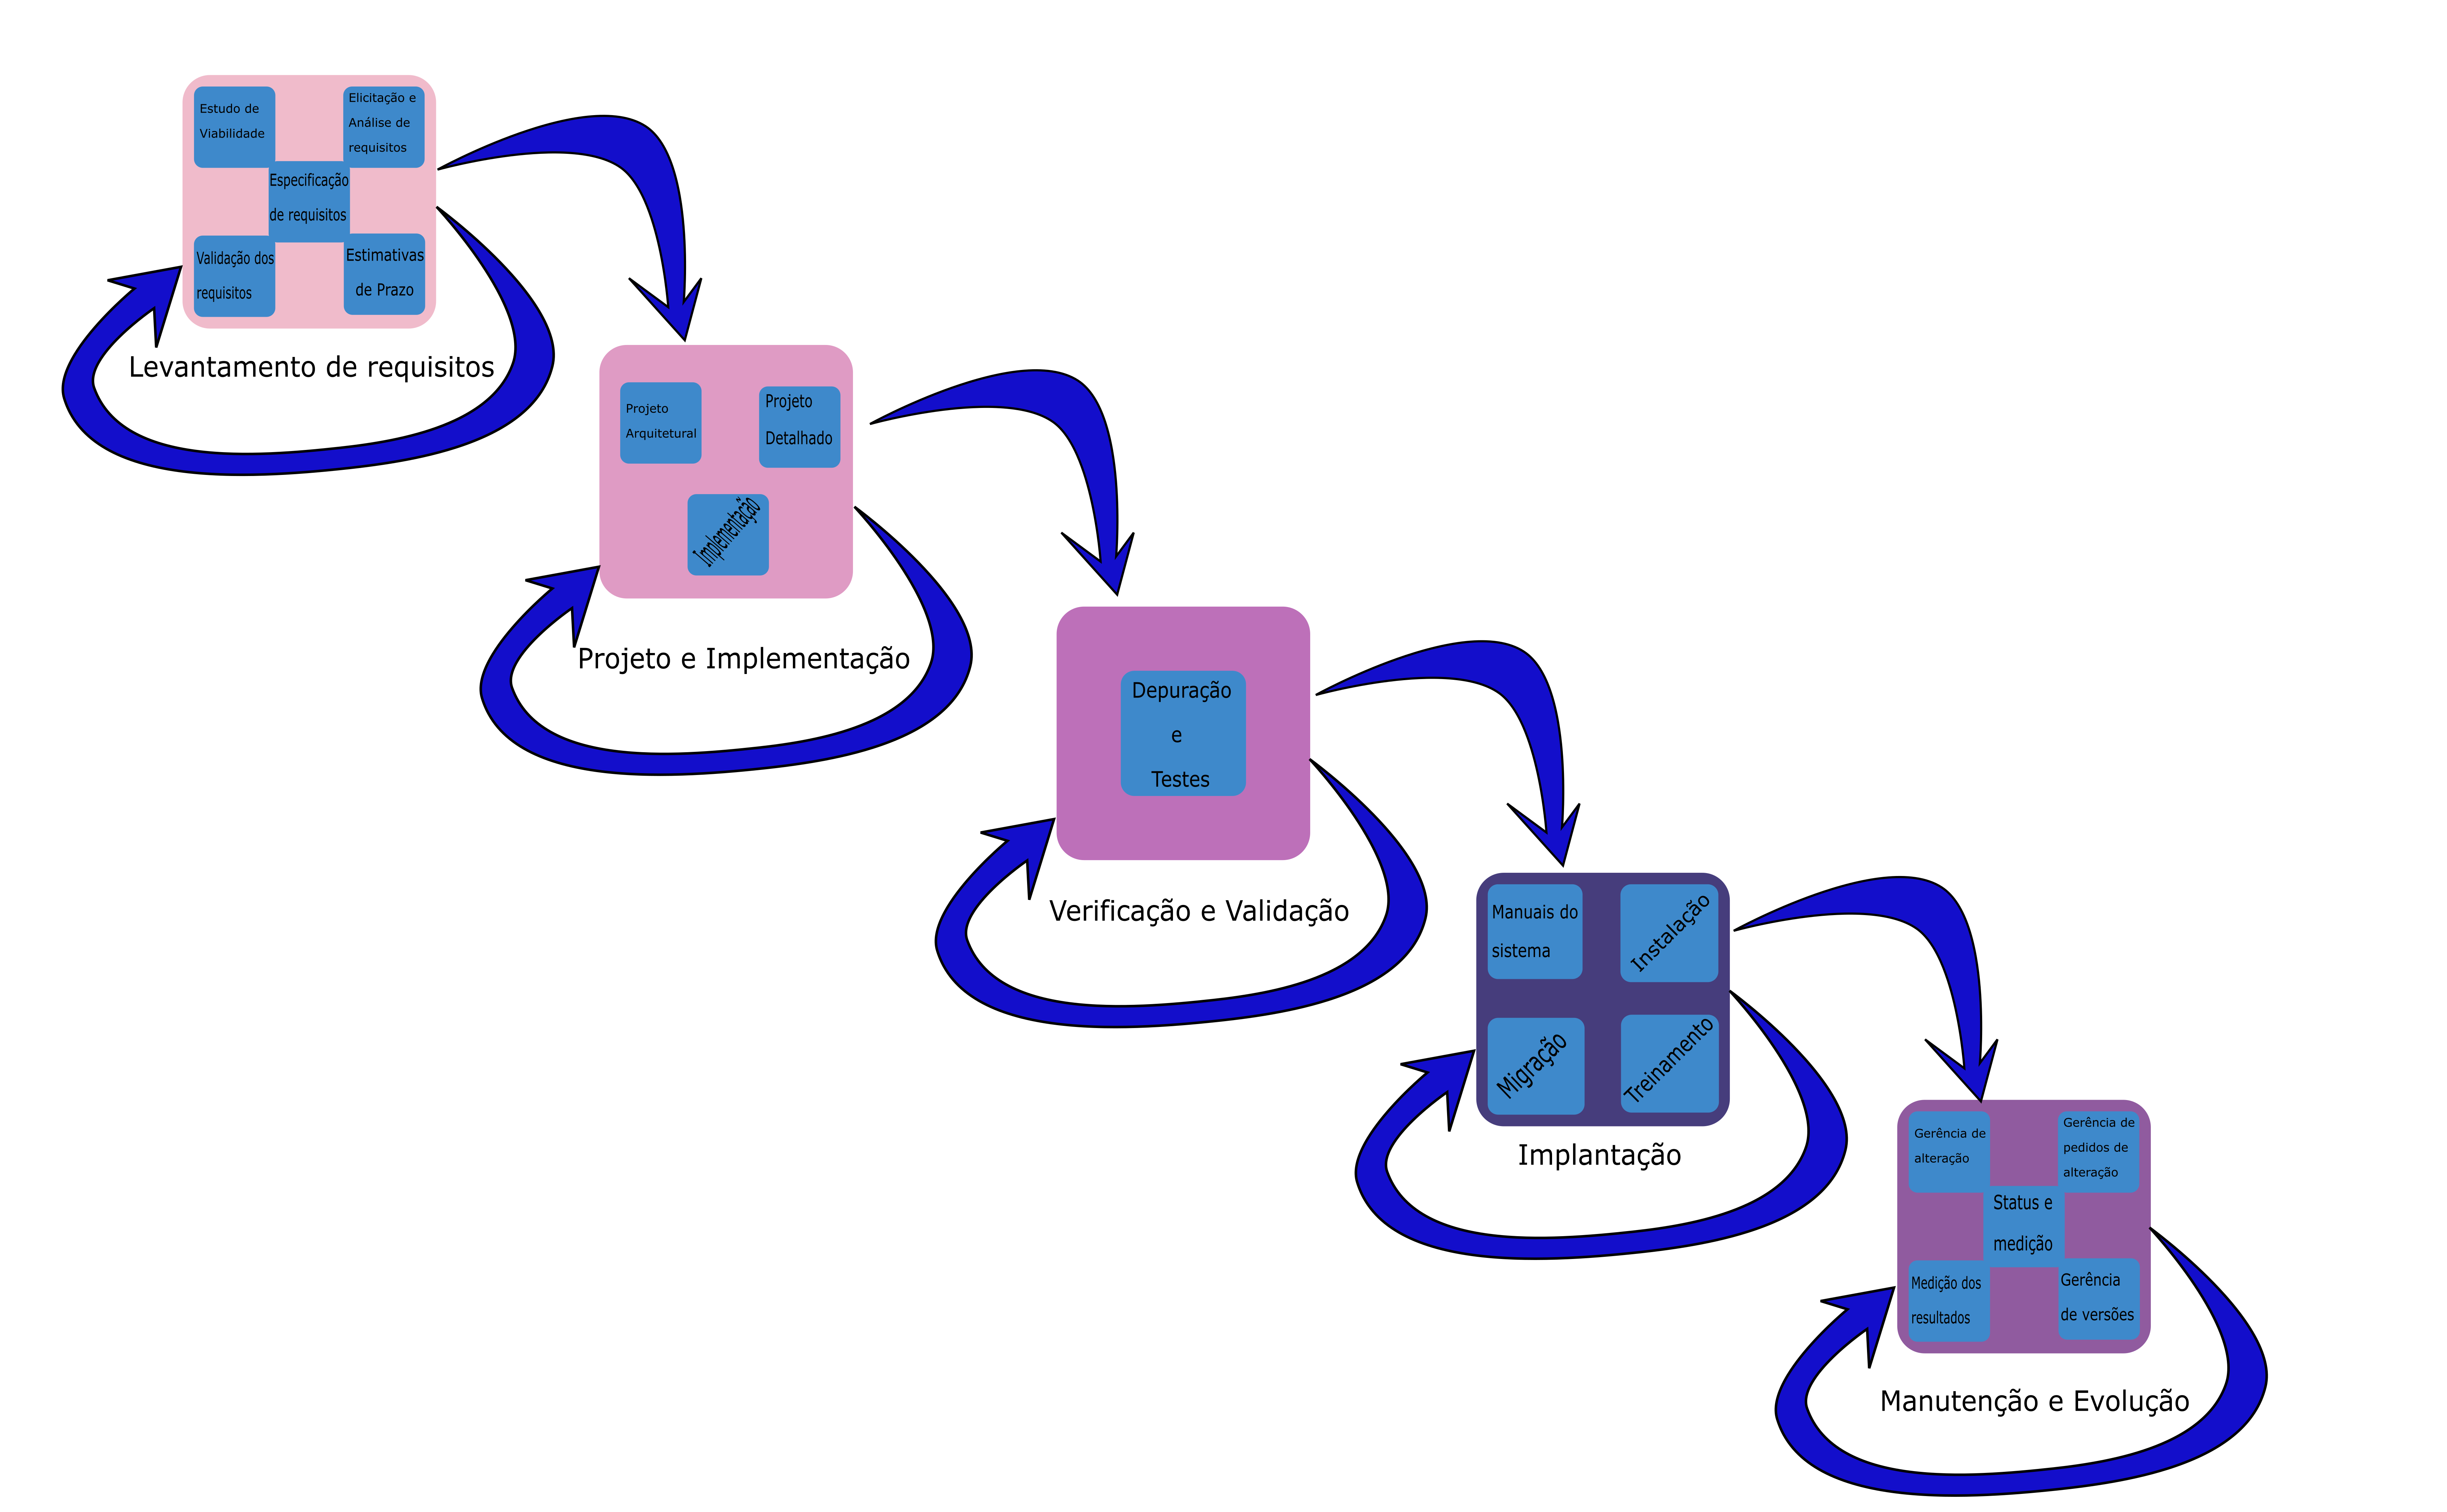
\includegraphics[width=\textwidth]{modelo-do-processo.png}
\caption{Modelo do Processo}
\label{modelodoprocesso}
\end{figure}
\FloatBarrier

O BPMN é o Modelo e Notação de Processos de Negócio que permite visualizar o gerenciamento dos processos de negócio do projeto que será desenvolvido. Os modelos foram divididos por fases, como podemos observar nas imagens abaixo.


\begin{figure}
\centering
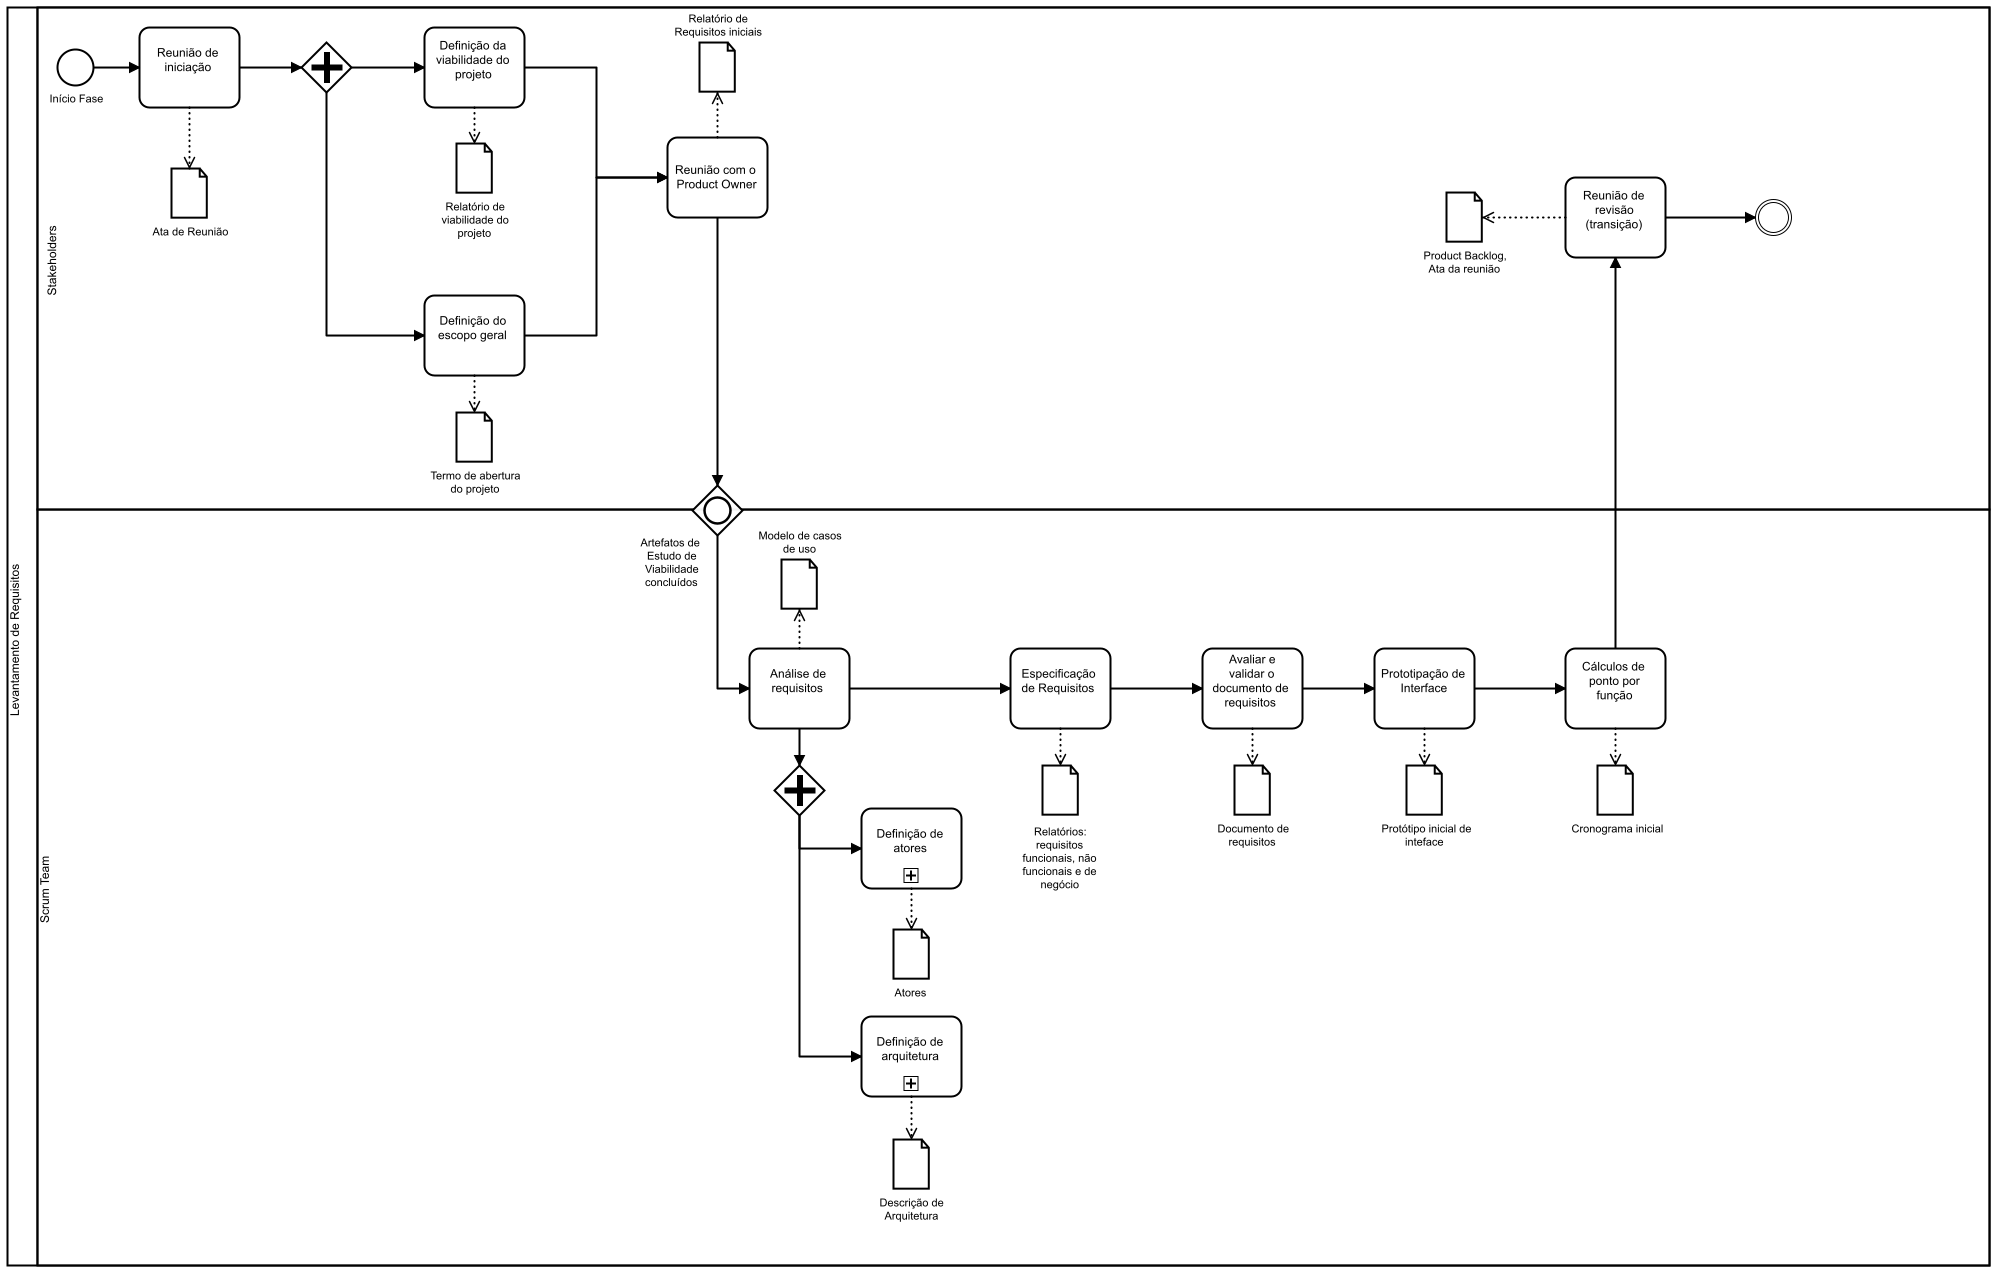
\includegraphics[width=\textwidth]{glevantamento.png}
\caption{Diagrama BPMN: Levantamento de Requisitos}
\label{levantamento}
\end{figure}
\FloatBarrier

\begin{figure}
\centering
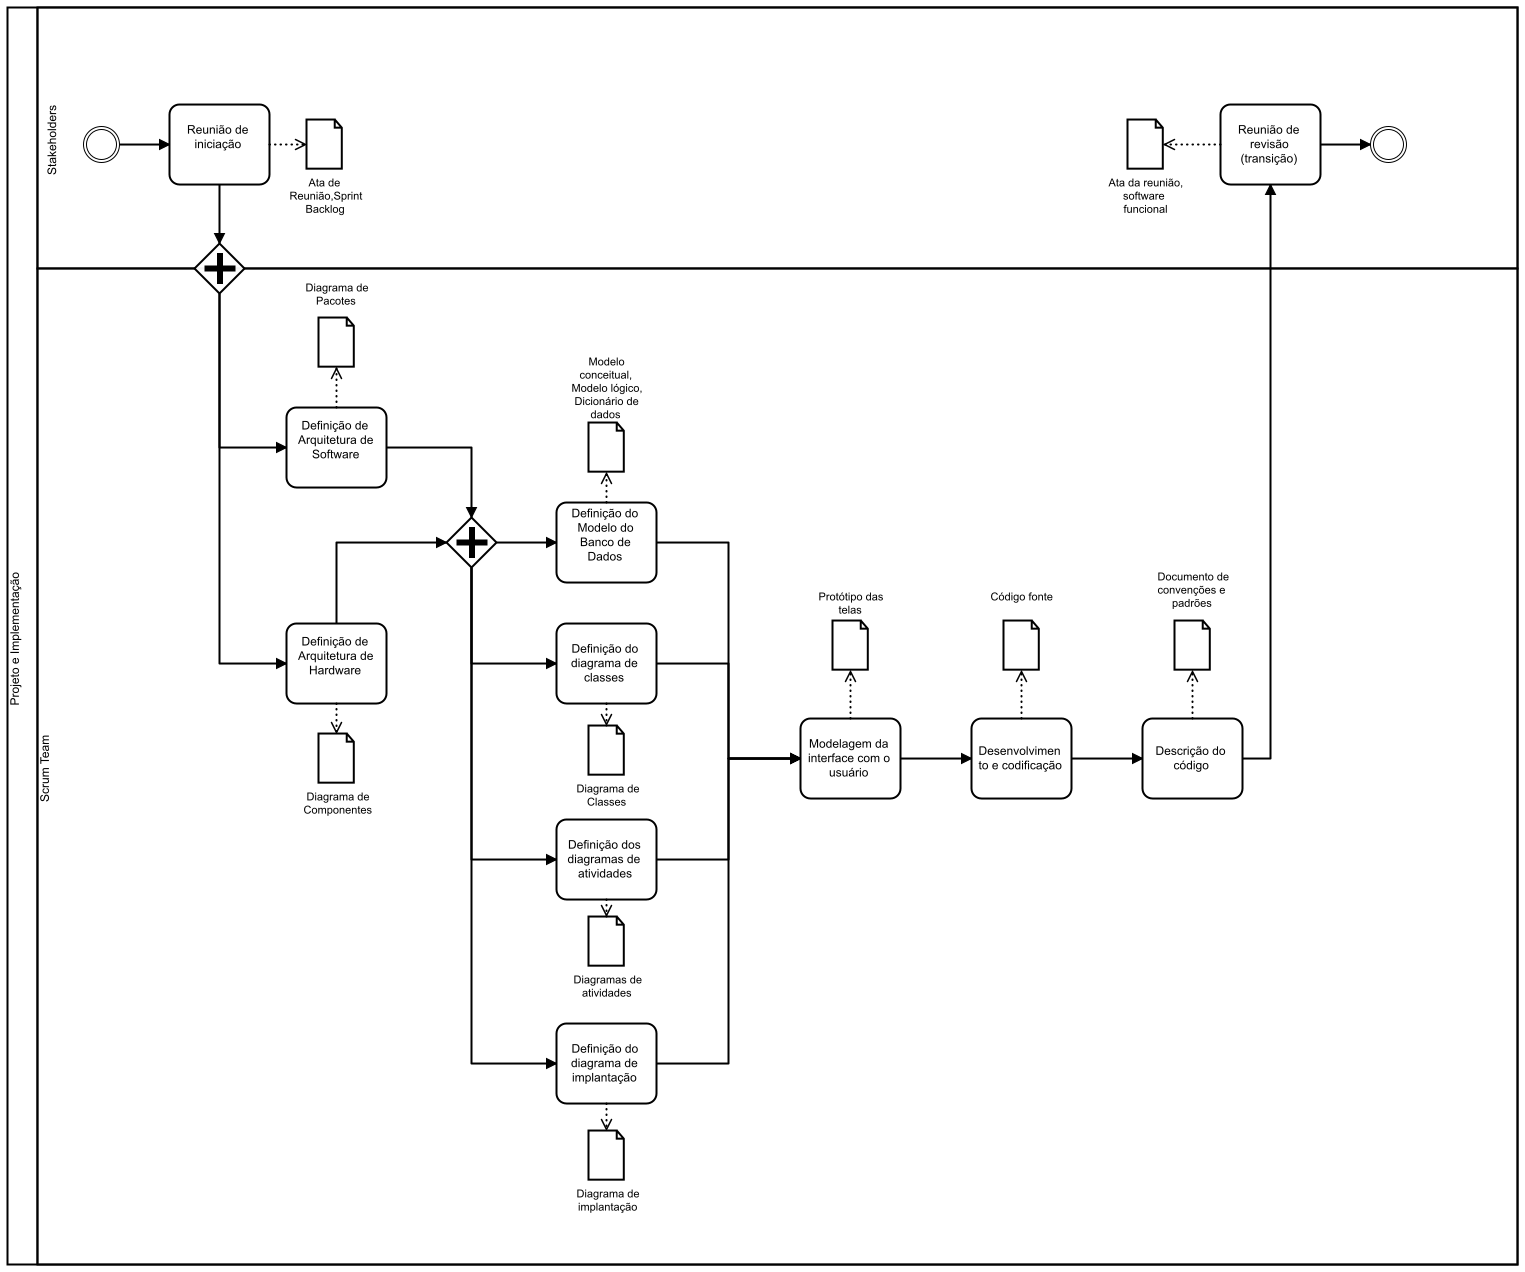
\includegraphics[width=\textwidth]{projeto_implementacao.png}
\caption{Diagrama BPMN: Projeto e Implementação}
\label{projeto}
\end{figure}
\FloatBarrier

\begin{figure}
\centering
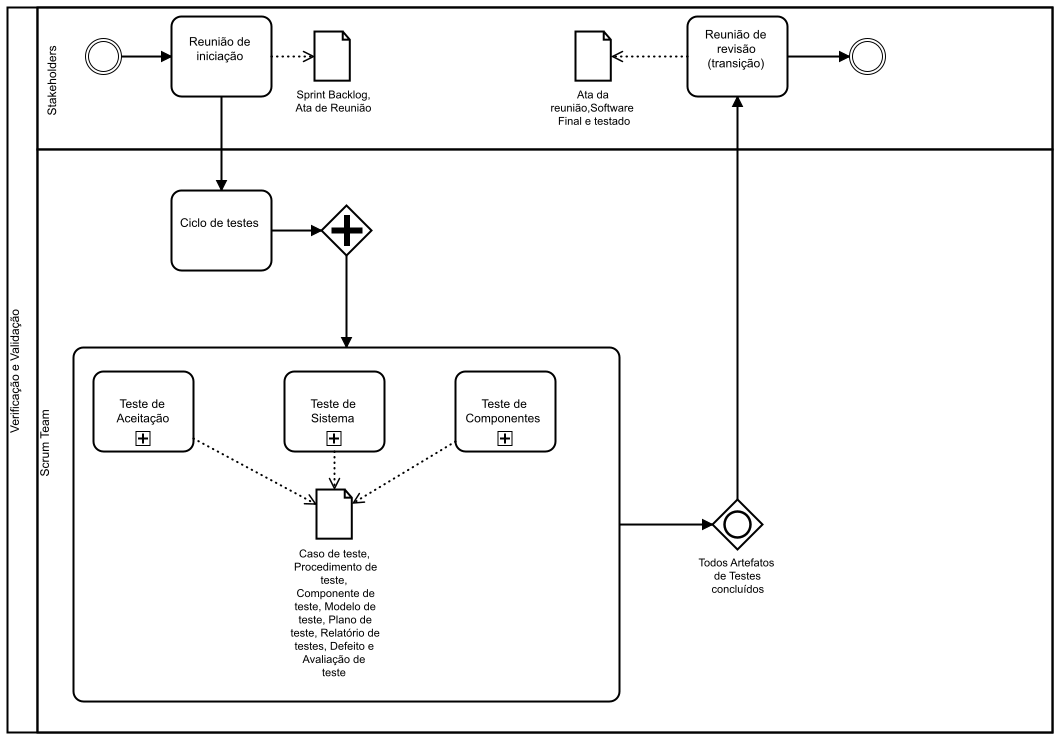
\includegraphics[width=\textwidth]{verificacao.png}
\caption{Diagrama BPMN: Verificação e validação}
\label{verificacao}
\end{figure}
\FloatBarrier

\begin{figure}
\centering
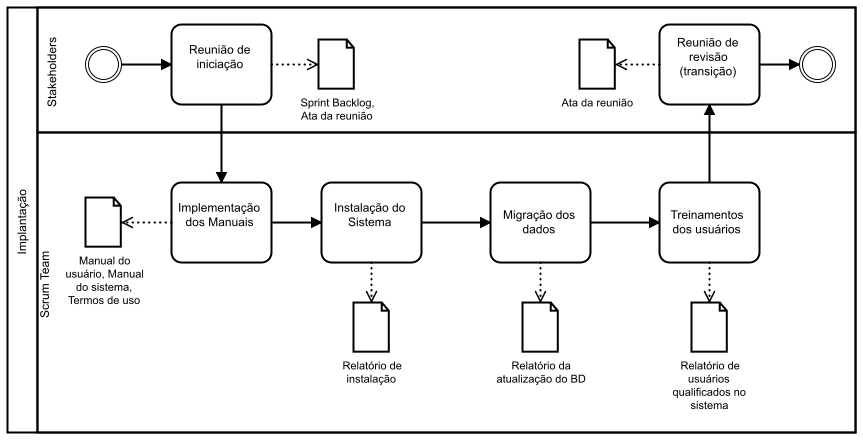
\includegraphics[width=\textwidth]{implantacaoo.png}
\caption{Diagrama BPMN: Implantação}
\label{implantacacao}
\end{figure}


\begin{figure}
\centering
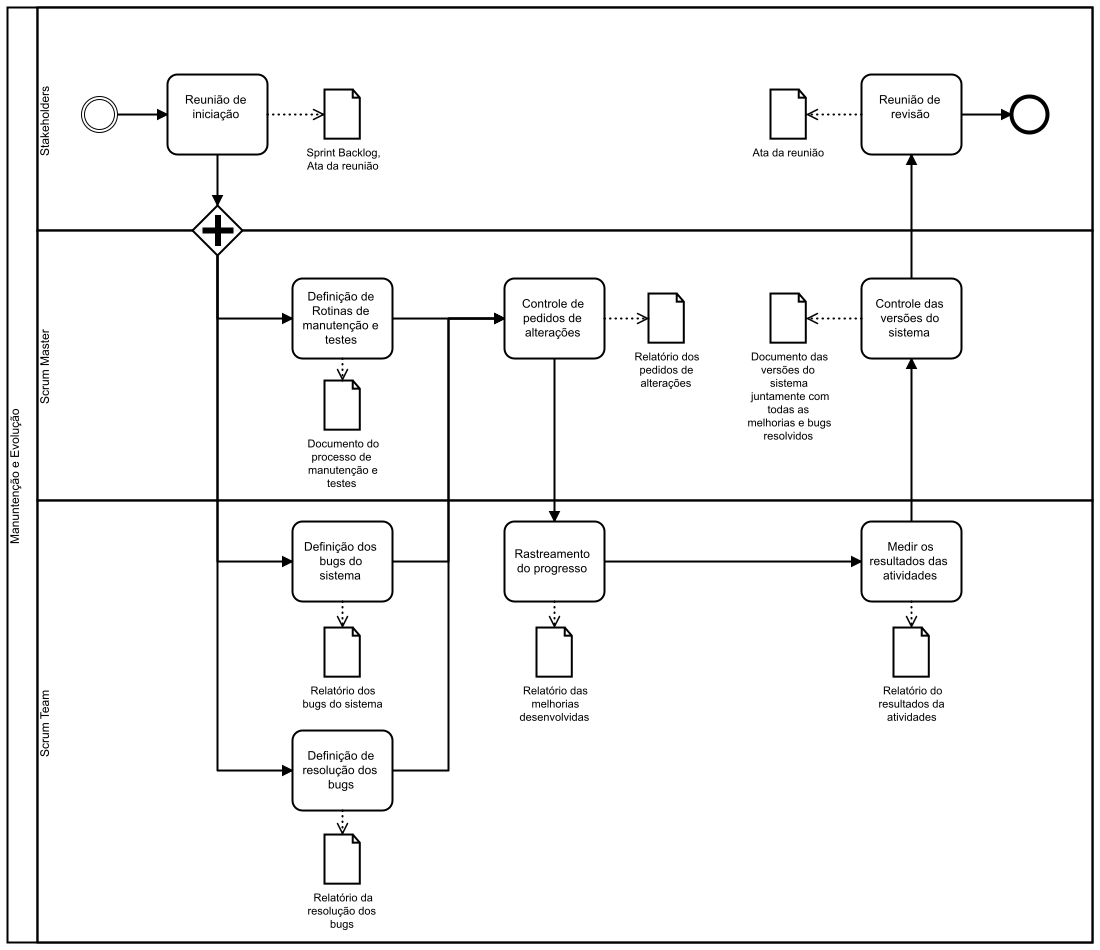
\includegraphics[width=\textwidth]{manutencao-evolucao.png}
\caption{Diagrama BPMN: Manutenção e Evolução}
\label{manutencao}
\end{figure}
\FloatBarrier




\subsection{Papeis}
No projeto foram utilizados os papéis da metodologia Scrum, onde são divididos em Product Owner, Scrum Master e Scrum Team. O Product Owner seria aquele que possui conhecimento dos requisitos do projeto, no caso o sujeito que deseja o sistema. Já o Scrum Master pode ser exercido por qualquer pessoa da equipe e é responsável por garantir que processo seja seguido e prever possíveis entraves que possam acarretar em atrasos no cronograma. No papel de Scrum Team os integrantes são flexíveis e podem desenvolver em todas áreas do projeto. Para melhor especificação a Tabela \ref{tabPapeis} descreve cada função existente que será necessária no projeto.//


% Table generated by Excel2LaTeX from sheet 'Planilha1'

\begin{longtable}[c]{|p{13.335em}|p{17.22em}|p{3.335em}|}
    %%%
   %%%
  %%% firsthead -- essa seção aparece apenas no primeiro cabeçalho.
  %%%
  \caption{Tabela com descrição dos papeis\label{tabPapeis}} \\
  \hline
  {Função} & {Descrição} & {Código} \\
  \hline\hline
  \endfirsthead
  %%%
  %%% head -- essa seção aparece nos demais cabeçalhos.
  %%%
  \caption[]{Tabela com descrição dos papeis (continuação)} \\
  \hline
  {Função} & {Descrição} & {Código} \\
  \hline\hline
  \endhead
    Gerente de projeto & Responsável por alocar recursos, garantir qualidade e integridade do sistema e definir prioridades & F01 \\
    \midrule
    Arquiteto de software & Responsável por definir interações do sistema, interfaces e por buscar soluções para problemas encontrados durante a construção do sistema & F02 \\
    \midrule
    Analista & Mão de obra principal, responsável pela escrita dos códigos e construção do sistema & F03 \\
    \midrule
    Engenheiro de Teste & Responsável por planejar os testes do sistema e avaliar os resultados posteriormente & F04 \\
    \midrule
    Tester & Responsável por efetuar os testes do sistema & F05 \\
    \midrule
    Arquiteto de Banco de Dados & Define o tipo de banco de dados a ser implementado, bem como sua arquitetura & F06 \\
    \midrule
    Designer & Desenvolve a interface gráfica de acordo com os modelos definidos pelo projetista de interfaces. & F07 \\
    \midrule
    Projetista de Interfaces & Determina a forma visual dos elementos da interface gráfica do sistema. (Desenvolve protótipos de tela) & F08 \\
    \midrule
    Analista de Requisitos & Responsável por mapear os requisitos ditos pelos stakeholders, mapear outros requisitos que irão aperfeiçoar o processo de desenvolvimento. & F09 \\
    \bottomrule
\end{longtable}


\FloatBarrier


\subsection{Atividades}
A Tabela \ref{tabAtvPapeis} descreve cada uma das atividades do processo, relacionando com o respectivo papel responsável por sua execução. \\

% Table generated by Excel2LaTeX from sheet 'Planilha2'
    \begin{longtable}[c]{|p{1.89em}|p{13.555em}|p{17.61em}|p{6.22em}|}
    %%%
   %%%
  %%% firsthead -- essa seção aparece apenas no primeiro cabeçalho.
  %%%
  \caption{Enumeração e descrição das atividades vinculados com os papeis\label{tabAtvPapeis}} \\
  \hline
  {} & {ATIVIDADE} & {DESCRIÇÃO DE ATIVIDADES} & {PAPÉIS} \\
  \hline\hline
  \endfirsthead
  %%%
  %%% head -- essa seção aparece nos demais cabeçalhos.
  %%%
  \caption[]{Enumeração e descrição das atividades vinculados com os papeis (continuação)} \\
  \hline
  {} & {ATIVIDADE} & {DESCRIÇÃO DE ATIVIDADES} & {PAPÉIS} \\
  \hline\hline
  \endhead
 
    \textbf{1.1} & Reunião de iniciação & Reunião para marcar os encontros com os stakeholders para que todos saibam o que é esperado dessa primeira fase, serão definidos os tempos para a execução das sprints e como podem ser realizadas & Stakeholders \\
    \midrule
    \textbf{1.2} & Definição da viabilidade do projeto & Verificar que com o orçamento proposto e tecnologias prontas para serem utilizadas são suficientes para a execução do projeto & Stakeholders \\
    \midrule
    \textbf{1.3} & Definição de escopo geral & Definir linguagem, limites e restrições, que problemas que devem ser resolvidos e como serão resolvidos & Stakeholders \\
    \midrule
    \textbf{1.4} & Reunião com o Product Owner & Reunião para verificar se o cliente está de acordo com o escopo definido & Stakeholders \\
    \midrule
    \textbf{1.5} & Análise de requisitos & Onde serão realizados os modelos de casos de uso para auxiliar na análise dos requisitos necessários e verificar as atividades e funcionalidades que precisam estar presentes no software a ser desenvolvido & Scrum Team \\
    \midrule
    \textbf{1.6} & Definição dos atores & A partir dos casos de usos são listados e verificados os atores envolvidos no sistema & Scrum Team \\
    \midrule
    \textbf{1.7} & Definição da arquitetura & São especificados os casos de uso gerais sobre as funcionalidades essenciais do sistema & Scrum Team \\
    \midrule
    \textbf{1.8} & Especificação dos requisitos & Com as funcionalidades definidas os requisitos funcionais e não funcionais podem ser mais especificados com o fim de validar a necessidade, se não estão ambíguos, e se suprem as demandas & Scrum Team \\
    \midrule
    \textbf{1.9} & Avaliar e validar o documento de requisitos & A partir dos relatórios dos requisitos, os requisitos são analisados em busca de verificar se possuem rastreabilidade, se estão íntegros, correlacionados e se o documento de requisitos são & Stakeholders \\
    \midrule
    \textbf{1.10} & Prototipação de interface & Com o uso de um design sprint será feito o estudo de um planejamento sobre a interface gráfica do sistema, para certificar que todos os requisitos estarão sendo preenchidos & Scrum Team \\
    \midrule
    \textbf{1.11} & Cálculo de pontos por função & Com o uso dos caso de uso, será realizado um cronograma inicial para se obter uma estimativa de prazo de execução do projeto & Scrum Team \\
    \midrule
    \textbf{1.12} & Reunião de revisão (transição) & Reunião de revisão de fase onde é verificado se o planejado foi executado, se há necessidade de mudança na execuções das sprints antes do inicio da próxima fase. É também elaborado o product backlog a partir de tudo que foi elicitado e também definido suas prioridades & Stakeholders \\
    \midrule
    \textbf{2.1} & Reunião de iniciação & Definido o sprint backlog para que os parâmetros das sprints sejam passados para o scrum team & Stakeholders \\
    \midrule
    \textbf{2.2} & Definição da arquitetura de hardware & São definidos todos os componentes (entregas) referentes ao projeto & Scrum Team \\
    \midrule
    \textbf{2.3} & Definição da arquitetura de software & Através do diagrama de pacote são definidos como os pacotes serão estruturados dentro da arquitetura do sistema & Scrum Team \\
    \midrule
    \textbf{2.4} & Definição do modelo de banco de dados & Nessa atividade é estudado os itens que precisam estar no banco de dados, se será relacional ou não relacional, atributos, entidades, chaves e relacionamentos & Scrum Team \\
    \midrule
    \textbf{2.5} & Definição do diagrama de classes & Desenvolvimento dos diagramas de classes para que se tenha a visão geral e como as classes serão relacionadas umas com as outras, seus métodos e organização em relação aos objetos, além de separar elementos de design dos elementos de sistema & Scrum Team \\
    \midrule
    \textbf{2.6} & Definição dos diagramas de atividades & Definir o fluxo do funcionamento e controle das atividades realizadas pelo sistema e como se interligam & Scrum Team \\
    \midrule
    \textbf{2.7} & Definição do diagrama de implantação & Desenvolvimento do Diagrama de Implantação que especifica os requisitos mínimos para o funcionamento do sistema tais como as bibliotecas e softwares necessários, assim como as definições de hardware & Scrum Team \\
    \midrule
    \textbf{2.8} & Modelagem da interface com o usuário & Diagramação para planejamento da tela e disposição dos itens na interface e estudo de como o usuário pode ter uma boa experiencia de utilização. Usa como base o protótipo inicial porém na aplicação de heurísticas e experiencia de usuário' & Scrum Team \\
    \midrule
    \textbf{2.9} & Desenvolvimento e codificação & Codificação & Scrum Team \\
    \midrule
    \textbf{2.10} & Descrição do código & São documentadas as formas e padrões adotados na codificação, além de descrever determinados blocos de código-fonte & Scrum Team \\
    \midrule
    \textbf{2.11} & \multicolumn{1}{r|}{} & Reunião de revisão de fase onde é verificado se o planejado foi executado, se há necessidade de mudança na execuções das sprints antes do inicio da proxima fase. Se o software atende ao escopo especificado & Stakeholders \\
    \midrule
    \textbf{3.1} & \multicolumn{1}{r|}{} & Reunião de inicio de fase, onde será definido como serão realizados os testes & Stakeholders \\
    \midrule
    \textbf{3.2} & Ciclo de testes & \multirow{1}{r|} & Realização dos testes e correção no software, se necessário. Os testes devem ser relatados & Scrum Team \\
\cmidrule{1-2}\cmidrule{4-4}    \textbf{3.3} & Teste de Componentes & \multicolumn{1}{r|}{} & Scrum Team \\
\cmidrule{1-2}\cmidrule{4-4}    \textbf{3.4} & Teste de Sistema & \multicolumn{1}{r|}{} & Scrum Team \\
\cmidrule{1-2}\cmidrule{4-4}    \textbf{3.5} & Teste de Aceitação & \multicolumn{1}{r|}{} & Scrum Team \\
    \midrule
    \textbf{3.6} & Reunião de revisão (transição) & Reunião de finalização do software, realizada com os os stakeholders a fim de validar o sistema de acordo com o que era esperado & Stakeholders \\
    \midrule
    \textbf{4.1} & Reunião de iniciação & Reunião de inicio de fase, onde é passado aos stakeholders como serão os procedimentos finais de desenvolvimento e como deve ser documentado as atualizações do sistema & Stakeholders \\
    \midrule
    \textbf{4.2} & Implementação dos Manuais & Desenvolvimento dos Manuais do usuário e sistema para treinamento ou ajuda adicional para usuários, além do desenvolvimento dos Termos de Uso para o software & Scrum Team \\
    \midrule
    \textbf{4.3} & Instalação do sistema & Instalação do sistema no ambiente requisitado pelo Product Owner seguindo as especificações & Scrum Team \\
    \midrule
    \textbf{4.4} & Migração dos dados & Transferência de dados antigos para o banco de dados arquitetado resumindo no mesmo atualizado & Scrum Team \\
    \midrule
    \textbf{4.5} & Treinamentos dos usuários & Relatório de resultados do treinamento dos usuários que foram qualifiados para o uso do sistema & Scrum Team \\
    \midrule
    \textbf{4.6} & Reunião de revisão (finalização) & Documentar considerações levantadas na reunião sobre o desenvolvimento das sprints e se o produto final está conforme o TAP, se atende o escopo e se o cliente final necessita de mais alguma alteração & Stakeholders \\
    \midrule
    \textbf{5.1} & Reunião de iniciação & Reunião de inicio da fase de manutenção e melhorias no sistema, definindo como o cronograma de rotinas será feito e especificação de relatórios de melhorias e bugs encontrados & Stakeholders \\
    \midrule
    \textbf{5.2} & Definição de Rotinas de manutenção e testes & Definição do cronograma e finalidades de manutenção e testes do sistema & Scrum Master \\
    \midrule
    \textbf{5.3} & Definição dos bugs do sistema & Relatório geral com o status de cada bug (se foi ou não resolvido, como foi resolvido, descrição do bug) & Scrum Team \\
    \midrule
    \textbf{5.4} & Definição de resolução dos bugs & Relatório geral das resoluções dos bugs encontrados no sistema\newline{} & Scrum Team \\
    \midrule
    \textbf{5.5} & Controle de pedidos de alterações & Status de cada pedido, se a melhoria sera ou não desenvolvida & Scrum Master \\
    \midrule
    \textbf{5.6} & Rastreamento do progresso & Relatório geral com o status de cada melhoria desenvolvida e seus respectivos feedback & Scrum Team \\
    \midrule
    \textbf{5.7} & Medir os resultados das atividades & observações: serve para verificar se as atividades alcançaram realmente o objetivo delas & Scrum Team \\
    \midrule
    \textbf{5.8} & Controle das versões do sistema & Desenvolvimento do documento das versões com os Relatórios de melhorias e resoluções de bugs no sistema, obtendo um controle das versões do sistema & Scrum Master \\
    \midrule
    \textbf{5.9} & Reunião de revisão (transição) & Documentar considerações levantadas na reunião sobre o desenvolvimento das sprints & Stakeholders \\
    \bottomrule
    \end{longtable}

\FloatBarrier

\section{Execução do projeto}

Nesta seção descrevemos o cronograma previsto para o projeto e o estado atual do projeto.

\subsection{Backlog e sprints}
O cronograma da Tabela \ref{tabCronAtvInt} abrange todas as sprints que serão realizadas durante o desenvolvimento e as respectivas atividades que deverão ser executadas naquele período. Cada atividade tem como responsável um integrante do projeto. A duração total prevista da execução do processo é de 17 semanas.

% Table generated by Excel2LaTeX from sheet 'Planilha2'

% Table generated by Excel2LaTeX from sheet 'Planilha2'
    \begin{longtable}[c]{|p{2em}|p{15em}|p{3em}|p{4em}|}

    %%%
   %%%
  %%% firsthead -- essa seção aparece apenas no primeiro cabeçalho.
  %%%
  \caption{Cronograma com as atribuições aos integrantes\label{tabCronAtvInt}} \\
  \hline
  {Sprint} & {Atividade} & {Integrante} & {Duração} \\
  \hline\hline
  \endfirsthead
  %%%
  %%% head -- essa seção aparece nos demais cabeçalhos.
  %%%
  \caption[]{Cronograma com as atribuições aos integrantes (continuação)} \\
  \hline
  {Sprint} & {Atividade} & {Integrante} & {Duração} \\
  \hline\hline
  \endhead
    \multicolumn{1}{|c|}{\multirow{2}[4]{*}{Estudo de viabilidade}} & \multicolumn{1}{p{10.055em}|}{Definição da viabilidade do projeto} & \multicolumn{1}{p{5.89em}|}{Isabelle} & \multirow{10}[20]{*}{2 semanas} \\
\cmidrule{2-3}         & \multicolumn{1}{p{10.055em}|}{Definição do escopo geral} & \multicolumn{1}{p{5.89em}|}{Felipe} & \multicolumn{1}{c|}{} \\
\cmidrule{1-3}    \multicolumn{1}{|c|}{\multirow{4}[8]{*}{Elicitação e Análise de requisitos}} & \multicolumn{1}{p{10.055em}|}{Reunião com o Product Owner} & \multicolumn{1}{p{5.89em}|}{Isabelle} & \multicolumn{1}{c|}{} \\
\cmidrule{2-3}         & \multicolumn{1}{p{10.055em}|}{Definição dos atores} & \multicolumn{1}{p{5.89em}|}{Felipe} & \multicolumn{1}{c|}{} \\
\cmidrule{2-3}         & \multicolumn{1}{p{10.055em}|}{Análise de requisitos} & \multicolumn{1}{p{5.89em}|}{Isabelle} & \multicolumn{1}{c|}{} \\
\cmidrule{2-3}         & \multicolumn{1}{p{10.055em}|}{Definição da arquitetura} & \multicolumn{1}{p{5.89em}|}{Nathiely} & \multicolumn{1}{c|}{} \\
\cmidrule{1-3}    \multicolumn{1}{|p{9.11em}|}{Especificação de requisitos} & \multicolumn{1}{p{10.055em}|}{Especificação dos requisitos} & \multicolumn{1}{p{5.89em}|}{Isabelle} & \multicolumn{1}{c|}{} \\
\cmidrule{1-3}    \multicolumn{1}{|c|}{\multirow{2}[4]{*}{Validação dos requisitos}} & \multicolumn{1}{p{10.055em}|}{Prototipação de interface} & \multicolumn{1}{p{5.89em}|}{Raniel} & \multicolumn{1}{c|}{} \\
\cmidrule{2-3}         & \multicolumn{1}{p{10.055em}|}{Avaliar e validar o documento de requisitos} & \multicolumn{1}{p{5.89em}|}{Nathiely} & \multicolumn{1}{c|}{} \\
\cmidrule{1-3}    \multicolumn{1}{|p{9.11em}|}{Estimativas de Prazo} & \multicolumn{1}{p{10.055em}|}{Cálculo de pontos por função} & \multicolumn{1}{p{5.89em}|}{Lucas Tarumoto} & \multicolumn{1}{c|}{} \\
    \midrule
    \multicolumn{1}{|c|}{\multirow{2}[4]{*}{Projeto Arquitetural}} & \multicolumn{1}{p{10.055em}|}{Definição da arquitetura de hardware} & \multicolumn{1}{p{5.89em}|}{Lucas Freitas} & \multirow{5}[10]{*}{1 semanas} \\
\cmidrule{2-3}         & \multicolumn{1}{p{10.055em}|}{Definição da arquitetura de software} & \multicolumn{1}{p{5.89em}|}{Nathiely} & \multicolumn{1}{c|}{} \\
\cmidrule{1-3}    \multicolumn{1}{|c|}{\multirow{3}[6]{*}{Projeto Detalhado}} & \multicolumn{1}{p{10.055em}|}{Definição do modelo de banco de dados} & \multicolumn{1}{p{5.89em}|}{Lucas Tarumoto} & \multicolumn{1}{c|}{} \\
\cmidrule{2-3}         & \multicolumn{1}{p{10.055em}|}{Definição do diagrama de classes} & \multicolumn{1}{p{5.89em}|}{Lucas Freitas} & \multicolumn{1}{c|}{} \\
\cmidrule{2-3}         & \multicolumn{1}{p{10.055em}|}{Definição dos diagramas de atividades} & \multicolumn{1}{p{5.89em}|}{Felipe} & \multicolumn{1}{c|}{} \\
    \midrule
    \multicolumn{1}{|c|}{\multirow{3}[6]{*}{Implementação}} & \multicolumn{1}{p{10.055em}|}{Modelagem da interface com o usuário} & \multicolumn{1}{p{5.89em}|}{Lucas Tarumoto} & \multirow{3}[6]{*}{4 semanas} \\
\cmidrule{2-3}         & \multicolumn{1}{p{10.055em}|}{Descrição do código} & \multicolumn{1}{p{5.89em}|}{Nathiely} & \multicolumn{1}{c|}{} \\
\cmidrule{2-3}         & \multicolumn{1}{p{10.055em}|}{Desenvolvimento e codificação} & \multicolumn{1}{p{5.89em}|}{Raniel} & \multicolumn{1}{c|}{} \\
    \midrule
    \multicolumn{1}{|c|}{\multirow{4}[8]{*}{Depuração e Testes}} & \multicolumn{1}{p{10.055em}|}{Ciclo de testes} & \multicolumn{1}{p{5.89em}|}{Felipe} & \multirow{4}[8]{*}{2 semanas} \\
\cmidrule{2-3}         & \multicolumn{1}{p{10.055em}|}{Teste de Componentes} & \multicolumn{1}{p{5.89em}|}{Lucas Freitas} & \multicolumn{1}{c|}{} \\
\cmidrule{2-3}         & \multicolumn{1}{p{10.055em}|}{Teste de Sistema} & \multicolumn{1}{p{5.89em}|}{Nathiely} & \multicolumn{1}{c|}{} \\
\cmidrule{2-3}         & \multicolumn{1}{p{10.055em}|}{Teste de Aceitação} & \multicolumn{1}{p{5.89em}|}{Raniel} & \multicolumn{1}{c|}{} \\
    \midrule
    \multicolumn{1}{|c|}{\multirow{4}[8]{*}{Implantação}} & \multicolumn{1}{p{10.055em}|}{Manuais do sistema} & \multicolumn{1}{p{5.89em}|}{Lucas Tarumoto} & \multirow{4}[8]{*}{2 semanas} \\
\cmidrule{2-3}         & \multicolumn{1}{p{10.055em}|}{Instalação} & \multicolumn{1}{p{5.89em}|}{Lucas Freitas} & \multicolumn{1}{c|}{} \\
\cmidrule{2-3}         & \multicolumn{1}{p{10.055em}|}{Migração} & \multicolumn{1}{p{5.89em}|}{Nathiely} & \multicolumn{1}{c|}{} \\
\cmidrule{2-3}         & \multicolumn{1}{p{10.055em}|}{Treinamento} & \multicolumn{1}{p{5.89em}|}{Felipe} & \multicolumn{1}{c|}{} \\
    \midrule
    \multicolumn{1}{|c|}{\multirow{3}[6]{*}{Gerência de alteração}} & \multicolumn{1}{p{10.055em}|}{Definição de Rotinas de manutenção e testes} & \multicolumn{1}{p{5.89em}|}{Raniel} & \multirow{3}[6]{*}{2 semanas} \\
\cmidrule{2-3}         & \multicolumn{1}{p{10.055em}|}{Definição dos bugs do sistema} & \multicolumn{1}{p{5.89em}|}{Felipe} & \multicolumn{1}{c|}{} \\
\cmidrule{2-3}         & \multicolumn{1}{p{10.055em}|}{Definição de resolução dos bugs} & \multicolumn{1}{p{5.89em}|}{Isabelle} & \multicolumn{1}{c|}{} \\
    \midrule
    \multicolumn{1}{|p{9.11em}|}{Gerência de pedidos de alteração} & \multicolumn{1}{p{10.055em}|}{Controle de pedidos de alterações} & \multicolumn{1}{p{5.89em}|}{Lucas Freitas} & Acompanha o projeto após o sistema ser liberado \\
    \midrule
    \multicolumn{1}{|p{9.11em}|}{Status e medição} & \multicolumn{1}{p{10.055em}|}{Rastreamento do progresso} & \multicolumn{1}{p{5.89em}|}{Lucas Tarumoto} & Acompanha o desenvolvimento \\
    \midrule
    \multicolumn{1}{|p{9.11em}|}{Medição dos resultados} & \multicolumn{1}{p{10.055em}|}{Medir os resultados das atividades} & \multicolumn{1}{p{5.89em}|}{Lucas Freitas} & Acompanha o desenvolvimento \\
    \midrule
    \multicolumn{1}{|p{9.11em}|}{Gerência de versões} & \multicolumn{1}{p{10.055em}|}{Controle das versões do sistema} & \multicolumn{1}{p{5.89em}|}{Lucas Tarumoto} & Acompanha desenvolvimento e a evolução do sistema \\
    \midrule
         &      &      & 13 semanas \\
    \bottomrule

 
\end{longtable}%

\FloatBarrier

\subsection{Estado atual}
Para o controle dos artefatos gerados pelo processo e das atividades de cada fase foram utilizados os templates abaixo, que têm por objetivo facilitar a visualização do estado atual do projeto, por meio de checklists.

O template da Tabela \ref{tabChecklistArtefato} é o checklist de todos os artefatos divididos por fases.

O template da Tabela \ref{tabChecklistAtividade} é o checklist de todas as atividades divididas por fases.

Ambas as tabelas foram ordenadas por ordem cronológica, facilitando a visualização de quais artefatos ou atividades já foram realizadas e quais ainda precisam ser entregues.

% Table generated by Excel2LaTeX from sheet 'Planilha4'
\begin{longtable}[c|]{|p{25.89em}|}
    %%%
   %%%
  %%% firsthead -- essa seção aparece apenas no primeiro cabeçalho.
  %%%
  \caption{Tabela de Checklist de Artefatos\label{tabChecklistArtefato}} \\
  \endfirsthead
  %%%
  %%% head -- essa seção aparece nos demais cabeçalhos.
  %%%
  \caption[]{Tabela de Checklist de Artefatos (continuação)} \\
  \midrule
  \endhead
  \toprule
    \multicolumn{2}{|p{25.11em}|}{\textbf{Levantamento de Requisitos }} \\
    \midrule
          & ( ) Ata de Reunião \\
    \midrule
          & ( ) Relatório da viabilidade do projeto \\
    \midrule
          & ( ) Termo de Abertura do Projeto \\
    \midrule
          & ( ) Relatório de Requisitos iniciais \\
    \midrule
          & ( ) Modelo de casos de uso \\
    \midrule
          & ( ) Atores \\
    \midrule
          & ( ) Descrição da arquitetura \\
    \midrule
          & ( ) Relatórios: requisitos funcionais, não funcionais e de negócio \\
    \midrule
          & ( ) Documento de Requisitos \\
    \midrule
          & ( ) Protótipo Inicial de interface \\
    \midrule
          & ( ) Cronograma inicial \\
    \midrule
          & ( ) Product Backlog, Ata da reunião \\
    \midrule
          & ( ) Ata de Reunião,Sprint Backlog \\
    \midrule
          & \textbf{Projeto e Implementação} \\
    \midrule
          & ( ) Diagrama de componentes \\
    \midrule
          & ( ) Diagrama de pacotes \\
    \midrule
          & ( ) Modelo conceitual, Modelo lógico, Dicionário de dados \\
    \midrule
          & ( ) Diagrama de classes \\
    \midrule
          & ( ) Diagramas de atividades \\
    \midrule
          & ( ) Diagrama de implantação \\
    \midrule
          & ( ) Protótipo das telas \\
    \midrule
          & ( ) Código fonte \\
    \midrule
          & ( ) Documento de convenções e padrões \\
    \midrule
          & ( ) Ata da reunião, software funcional \\
    \midrule
          & ( ) Sprint Backlog, Ata de Reunião \\
    \midrule
    \multicolumn{2}{|p{25.11em}|}{\textbf{Verificação e Validação}} \\
    \midrule
          & ( ) Caso de teste, Procedimento de teste, Componente de teste, Modelo de teste, Plano de teste, Relatório de testes, Defeito e Avaliação de teste (Teste de Componentes) \\
    \midrule
          & ( ) Caso de teste, Procedimento de teste, Componente de teste, Modelo de teste, Plano de teste, Relatório de testes, Defeito e Avaliação de teste (Teste de Sistema) \\
    \midrule
          & ( ) Caso de teste, Procedimento de teste, Componente de teste, Modelo de teste, Plano de teste, Relatório de testes, Defeito e Avaliação de teste (Teste de Aceitação) \\
    \midrule
          & ( ) Ata da reunião,Software Final e testado \\
    \midrule
          & ( ) Sprint Backlog, Ata da reunião \\
    \midrule
    \multicolumn{2}{|p{25.11em}|}{\textbf{Implantação}} \\
    \midrule
          & ( ) Manual do usuário, Manual do sistema, Termos de uso \\
    \midrule
          & ( ) Sistema instalado \\
    \midrule
          & ( ) Banco de dados atualizado \\
    \midrule
          & ( ) Relatório de usuários qualificados no sistema \\
    \midrule
          & ( ) Ata da reunião \\
    \midrule
          & ( ) Sprint Backlog, Ata da reunião \\
    \midrule
    \multicolumn{2}{|p{25.11em}|}{\textbf{Manutenção e Evolução}} \\
    \midrule
          & ( ) Documento do processo de manutenção e testes \\
    \midrule
          & ( ) Relatório dos bugs do sistema \\
    \midrule
          & ( ) Relatório da resolução dos bugs \\
    \midrule
          & ( ) Relatório dos pedidos de alterações \\
    \midrule
          & ( ) Relatório das melhorias desenvolvidas \\
    \midrule
          & ( ) Relatório do resultados da atividades \\
    \midrule
          & ( ) Documento das versões do sistema juntamente com todas as melhorias e bugs resolvidos \\
    \midrule
          & ( ) Ata da reunião \\
    \bottomrule
\end{longtable}

\FloatBarrier

% Table generated by Excel2LaTeX from sheet 'Planilha3'
\begin{longtable}[c|]{|p{25.89em}|}
    %%%
   %%%
  %%% firsthead -- essa seção aparece apenas no primeiro cabeçalho.
  %%%
  \caption{Tabela de Checklist de Atividades\label{tabChecklistAtividade}} \\
  \endfirsthead
  %%%
  %%% head -- essa seção aparece nos demais cabeçalhos.
  %%%
  \caption[]{Tabela de Checklist de Atividades (continuação)} \\
  \midrule
  \endhead
    \toprule
    \multicolumn{2}{}{\textbf{Levantamento de Requisitos }} \\
    \midrule
          & ( ) {Definição da viabilidade do projeto} \\
    \midrule
          & ( ) Definição de escopo geral \\
    \midrule
         & ( ) Reunião com o Product Owner \\
    \midrule
         & ( ) Análise de requisitos \\
    \midrule
          & ( ) Definição dos atores \\
    \midrule
          & ( ) Definição da arquitetura \\
    \midrule
          & ( ) Especificação dos requisitos \\
    \midrule
          & ( ) Avaliar e validar o documento de requisitos \\
    \midrule
          & ( ) Prototipação de interface \\
    \midrule
          & ( ) Cálculo de pontos por função \\
    \midrule
    \multicolumn{2}{|c|}{\textbf{Projeto e Implementação}} \\
    \midrule
          & ( ) Definição da arquitetura de hardware \\
    \midrule
          & ( ) Definição da arquitetura de software \\
    \midrule
          & ( ) Definição do modelo de banco de dados \\
    \midrule
          & ( ) Definição do diagrama de classes \\
    \midrule
          & ( ) Definição dos diagramas de atividades \\
    \midrule
          & ( ) Definição do diagrama de implantação \\
    \midrule
          & ( ) Modelagem da interface com o usuário \\
    \midrule
          & ( ) Desenvolvimento e codificação \\
    \midrule
          & ( ) Descrição do código \\
    \midrule
          & \multicolumn{1}{c|}{\textbf{Verificação e Validação}} \\
    \midrule
          & ( ) Ciclo de testes \\
    \midrule
          & ( ) Teste de Componentes \\
    \midrule
          & ( ) Teste de Sistema \\
    \midrule
          & ( ) Teste de Aceitação \\
    \midrule
    \multicolumn{2}{|c|}{\textbf{Implantação}} \\
    \midrule
          & ( ) Implementação dos Manuais \\
    \midrule
          & ( ) Instalação do sistema \\
    \midrule
          & ( ) Migração dos dados \\
    \midrule
          & ( ) Treinamentos dos usuários \\
    \midrule
          & ( ) Definição de Rotinas de manutenção e testes \\
    \midrule
          & ( ) Definição dos bugs do sistema \\
    \midrule
          & ( ) Definição de resolução dos bugs \\
    \midrule
    \multicolumn{2}{|c|}{\textbf{Manutenção e Evolução}} \\
    \midrule
          & ( ) Controle de pedidos de alterações \\
    \midrule
          & ( ) Rastreamento do progresso \\
    \midrule
          & ( ) Medir os resultados das atividades \\
    \midrule
          & ( ) Controle das versões do sistema \\
    \bottomrule
\end{longtable}




\FloatBarrier

Complementando, nos anexos possui os templates de relatórios Geral na figura \ref{relatorioGeral}, relatório de instalação na figura \ref{relatorioInstalacao},
template de finalização na figura \ref{templateFinalizacao}, template de Inicialização de Sprint na figura \ref{templateInicializacao} e Template de ata de reunião de definição de Sprints na figura \ref{templateSprint}


\section{Referências bibliográficas}
\renewcommand\refname{} %%Referências bibliográficas}  
\bibliographystyle{ieeetr}
\bibliography{bibliografia}  

\section{Anexos}
\begin{figure}
\centering
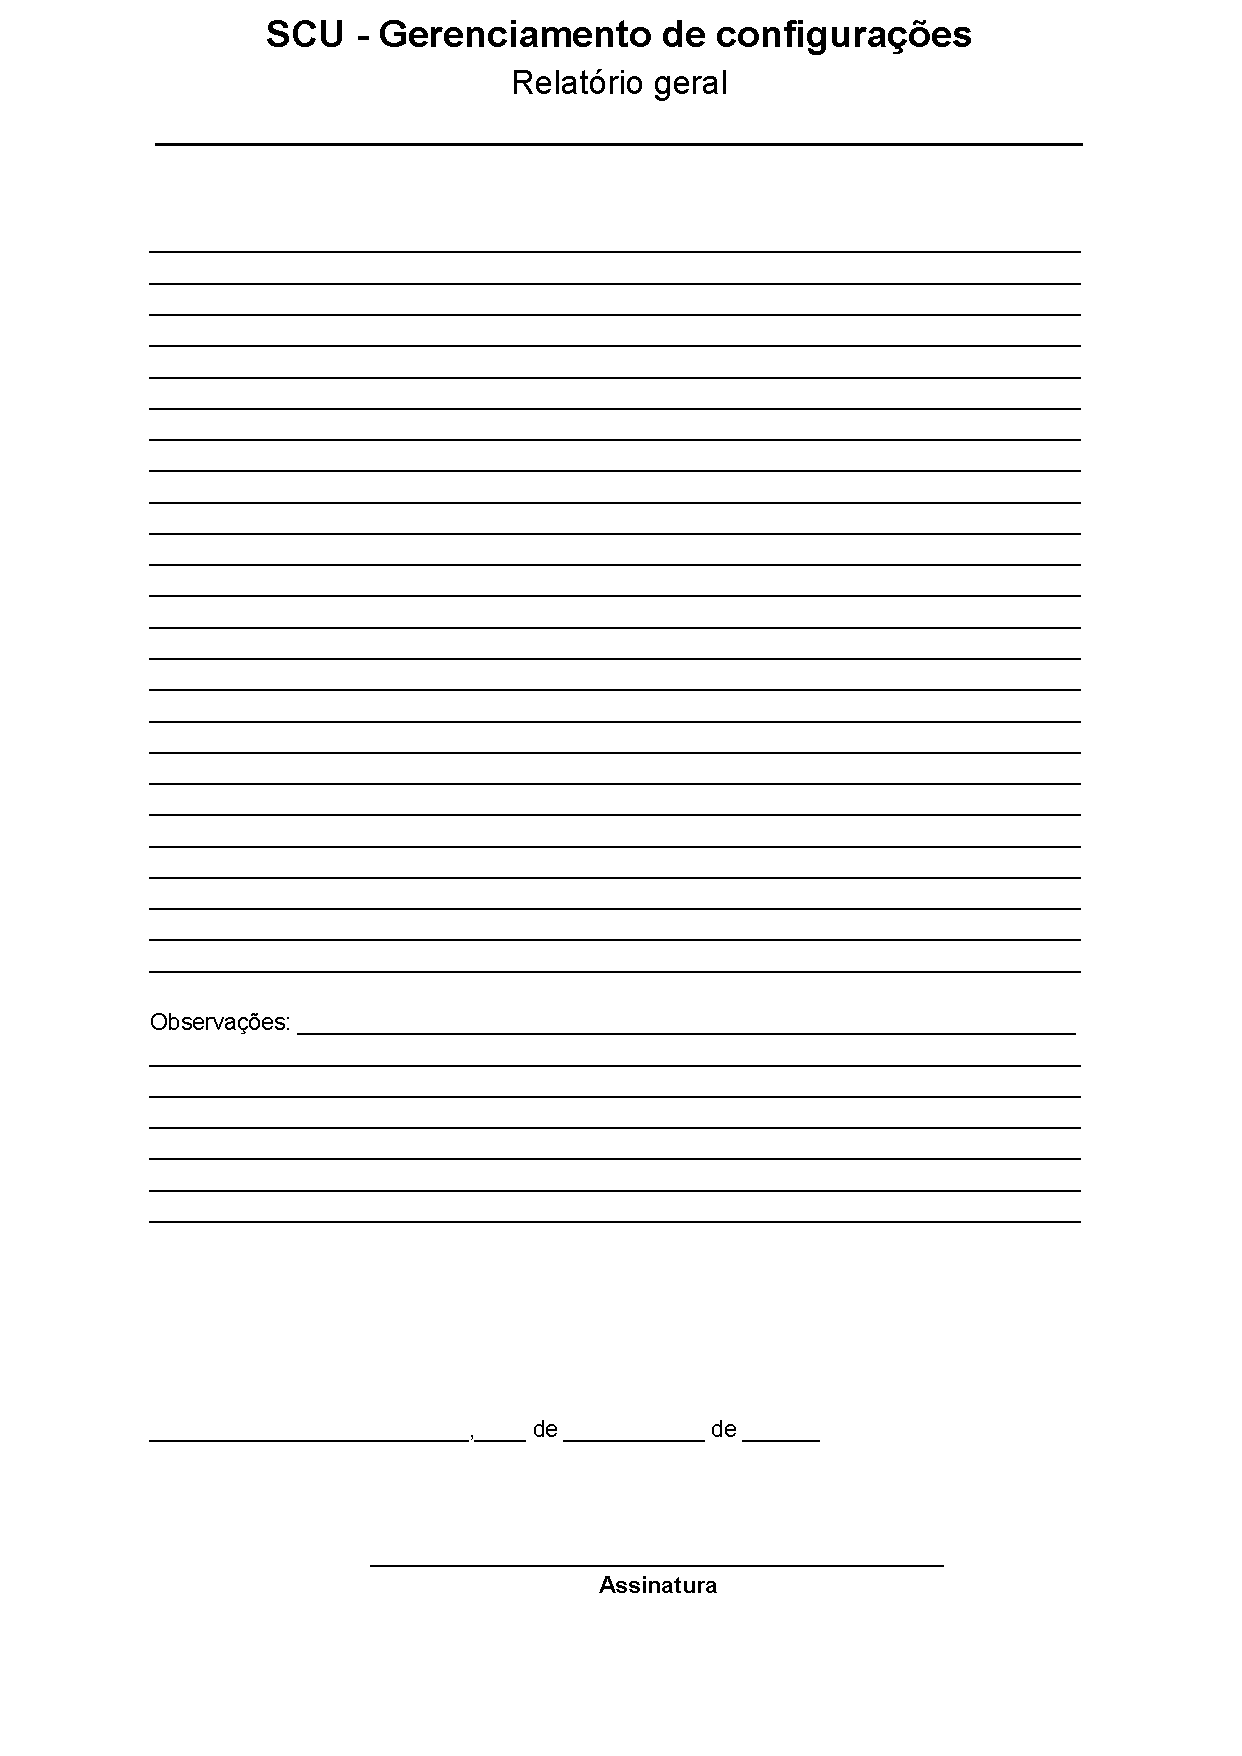
\includegraphics[width=\textwidth]{templateRel.pdf}
\caption{Template Relatório Geral}
\label{relatorioGeral}
\end{figure}
\FloatBarrier

\begin{figure}
\centering
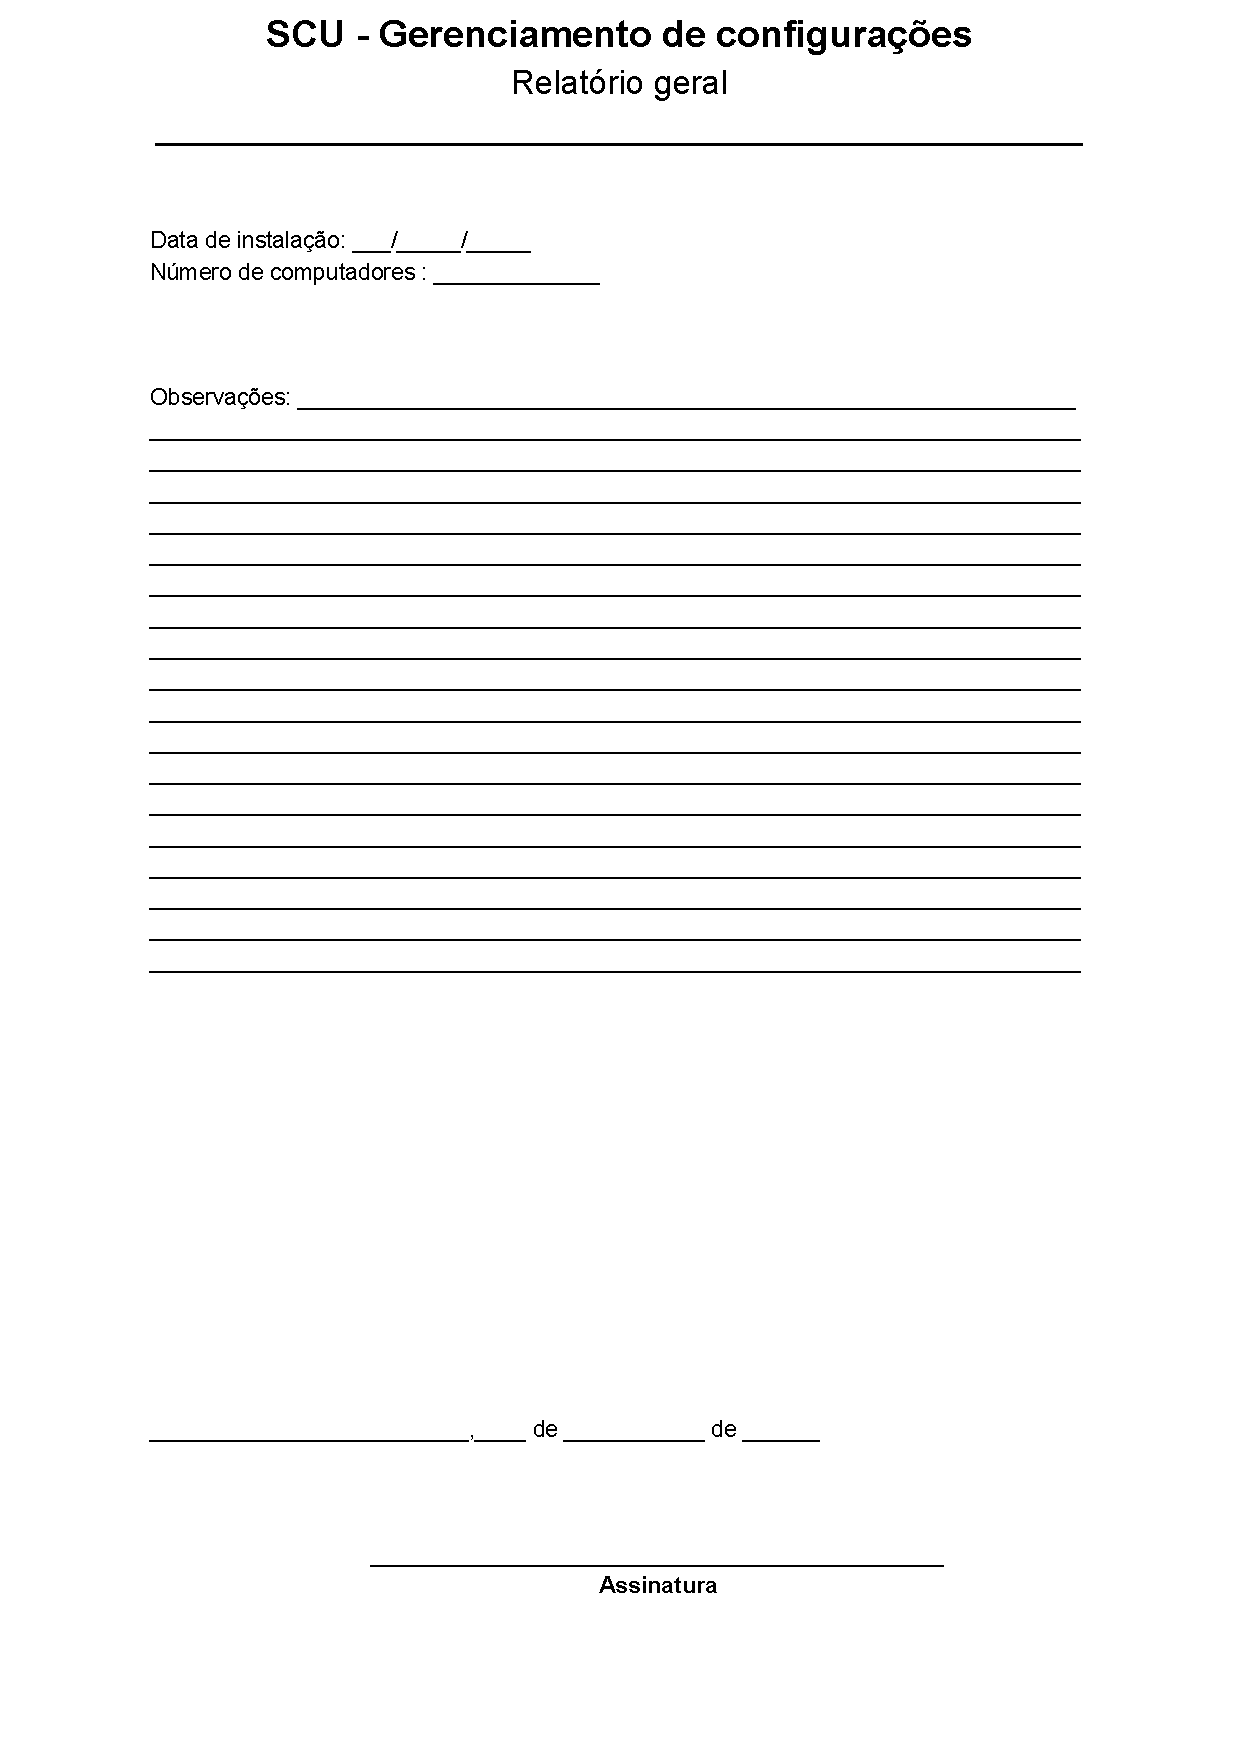
\includegraphics[width=\textwidth]{templateInstalacao.pdf}
\caption{Template de Relatório de Instalação}
\label{relatorioInstalacao}
\end{figure}
\FloatBarrier

\begin{figure}
\centering
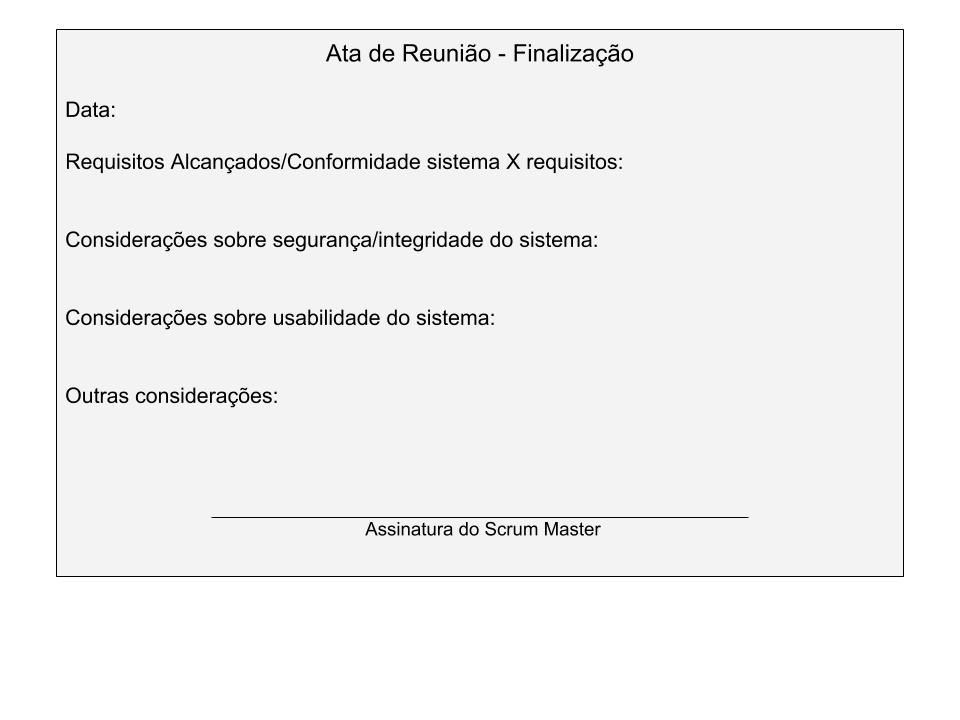
\includegraphics[width=\textwidth]{finalizacao.jpg}
\caption{Template ata de reunião de finalização de fase}
\label{templateFinalizacao}
\end{figure}
\FloatBarrier

\begin{figure}
\centering
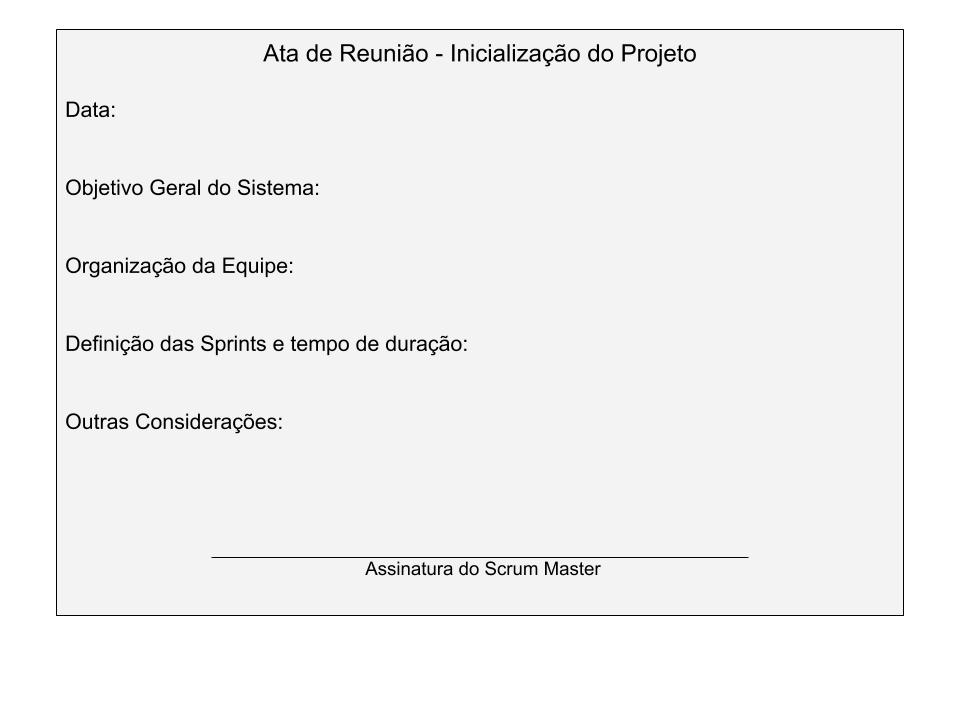
\includegraphics[width=\textwidth]{iniciacaoProjeto.jpg}
\caption{Template ata de reunião de incialização do Projeto}
\label{templateInicializacao}
\end{figure}
\FloatBarrier

\begin{figure}
\centering
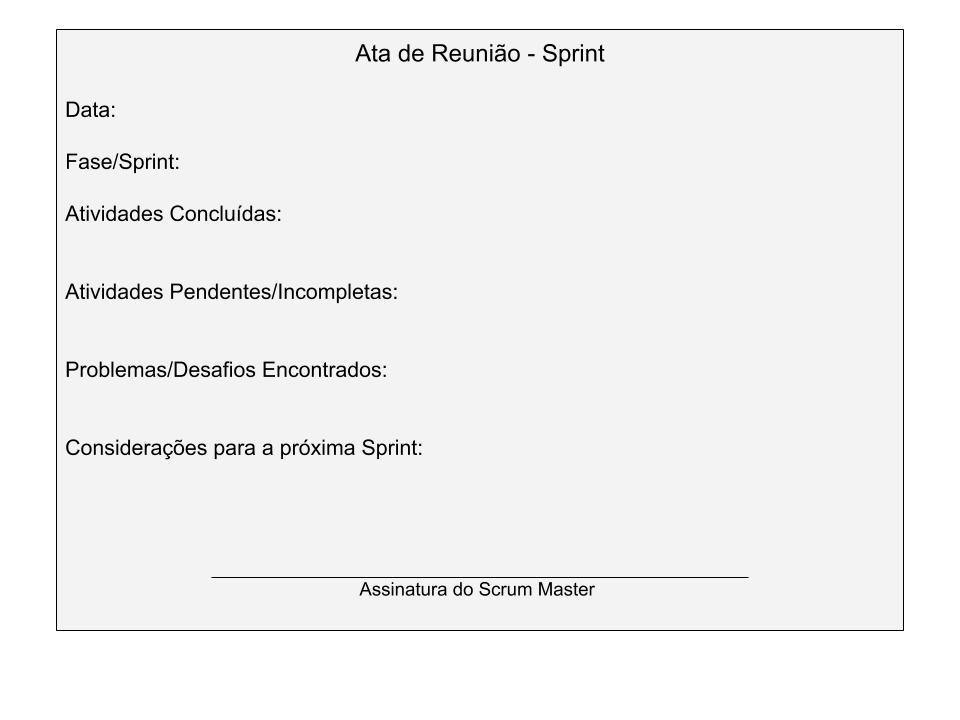
\includegraphics[width=\textwidth]{iniciacaoSprint.jpg}
\caption{Template ata de reunião de iniciação de Sprint}
\label{templateSprint}
\end{figure}
\FloatBarrier

\end{document}